\mysubsection{Alexander Scheurer und Sarah Häfele}{Vorgehen}

\begin{figure}[!htbp]
	\centering
		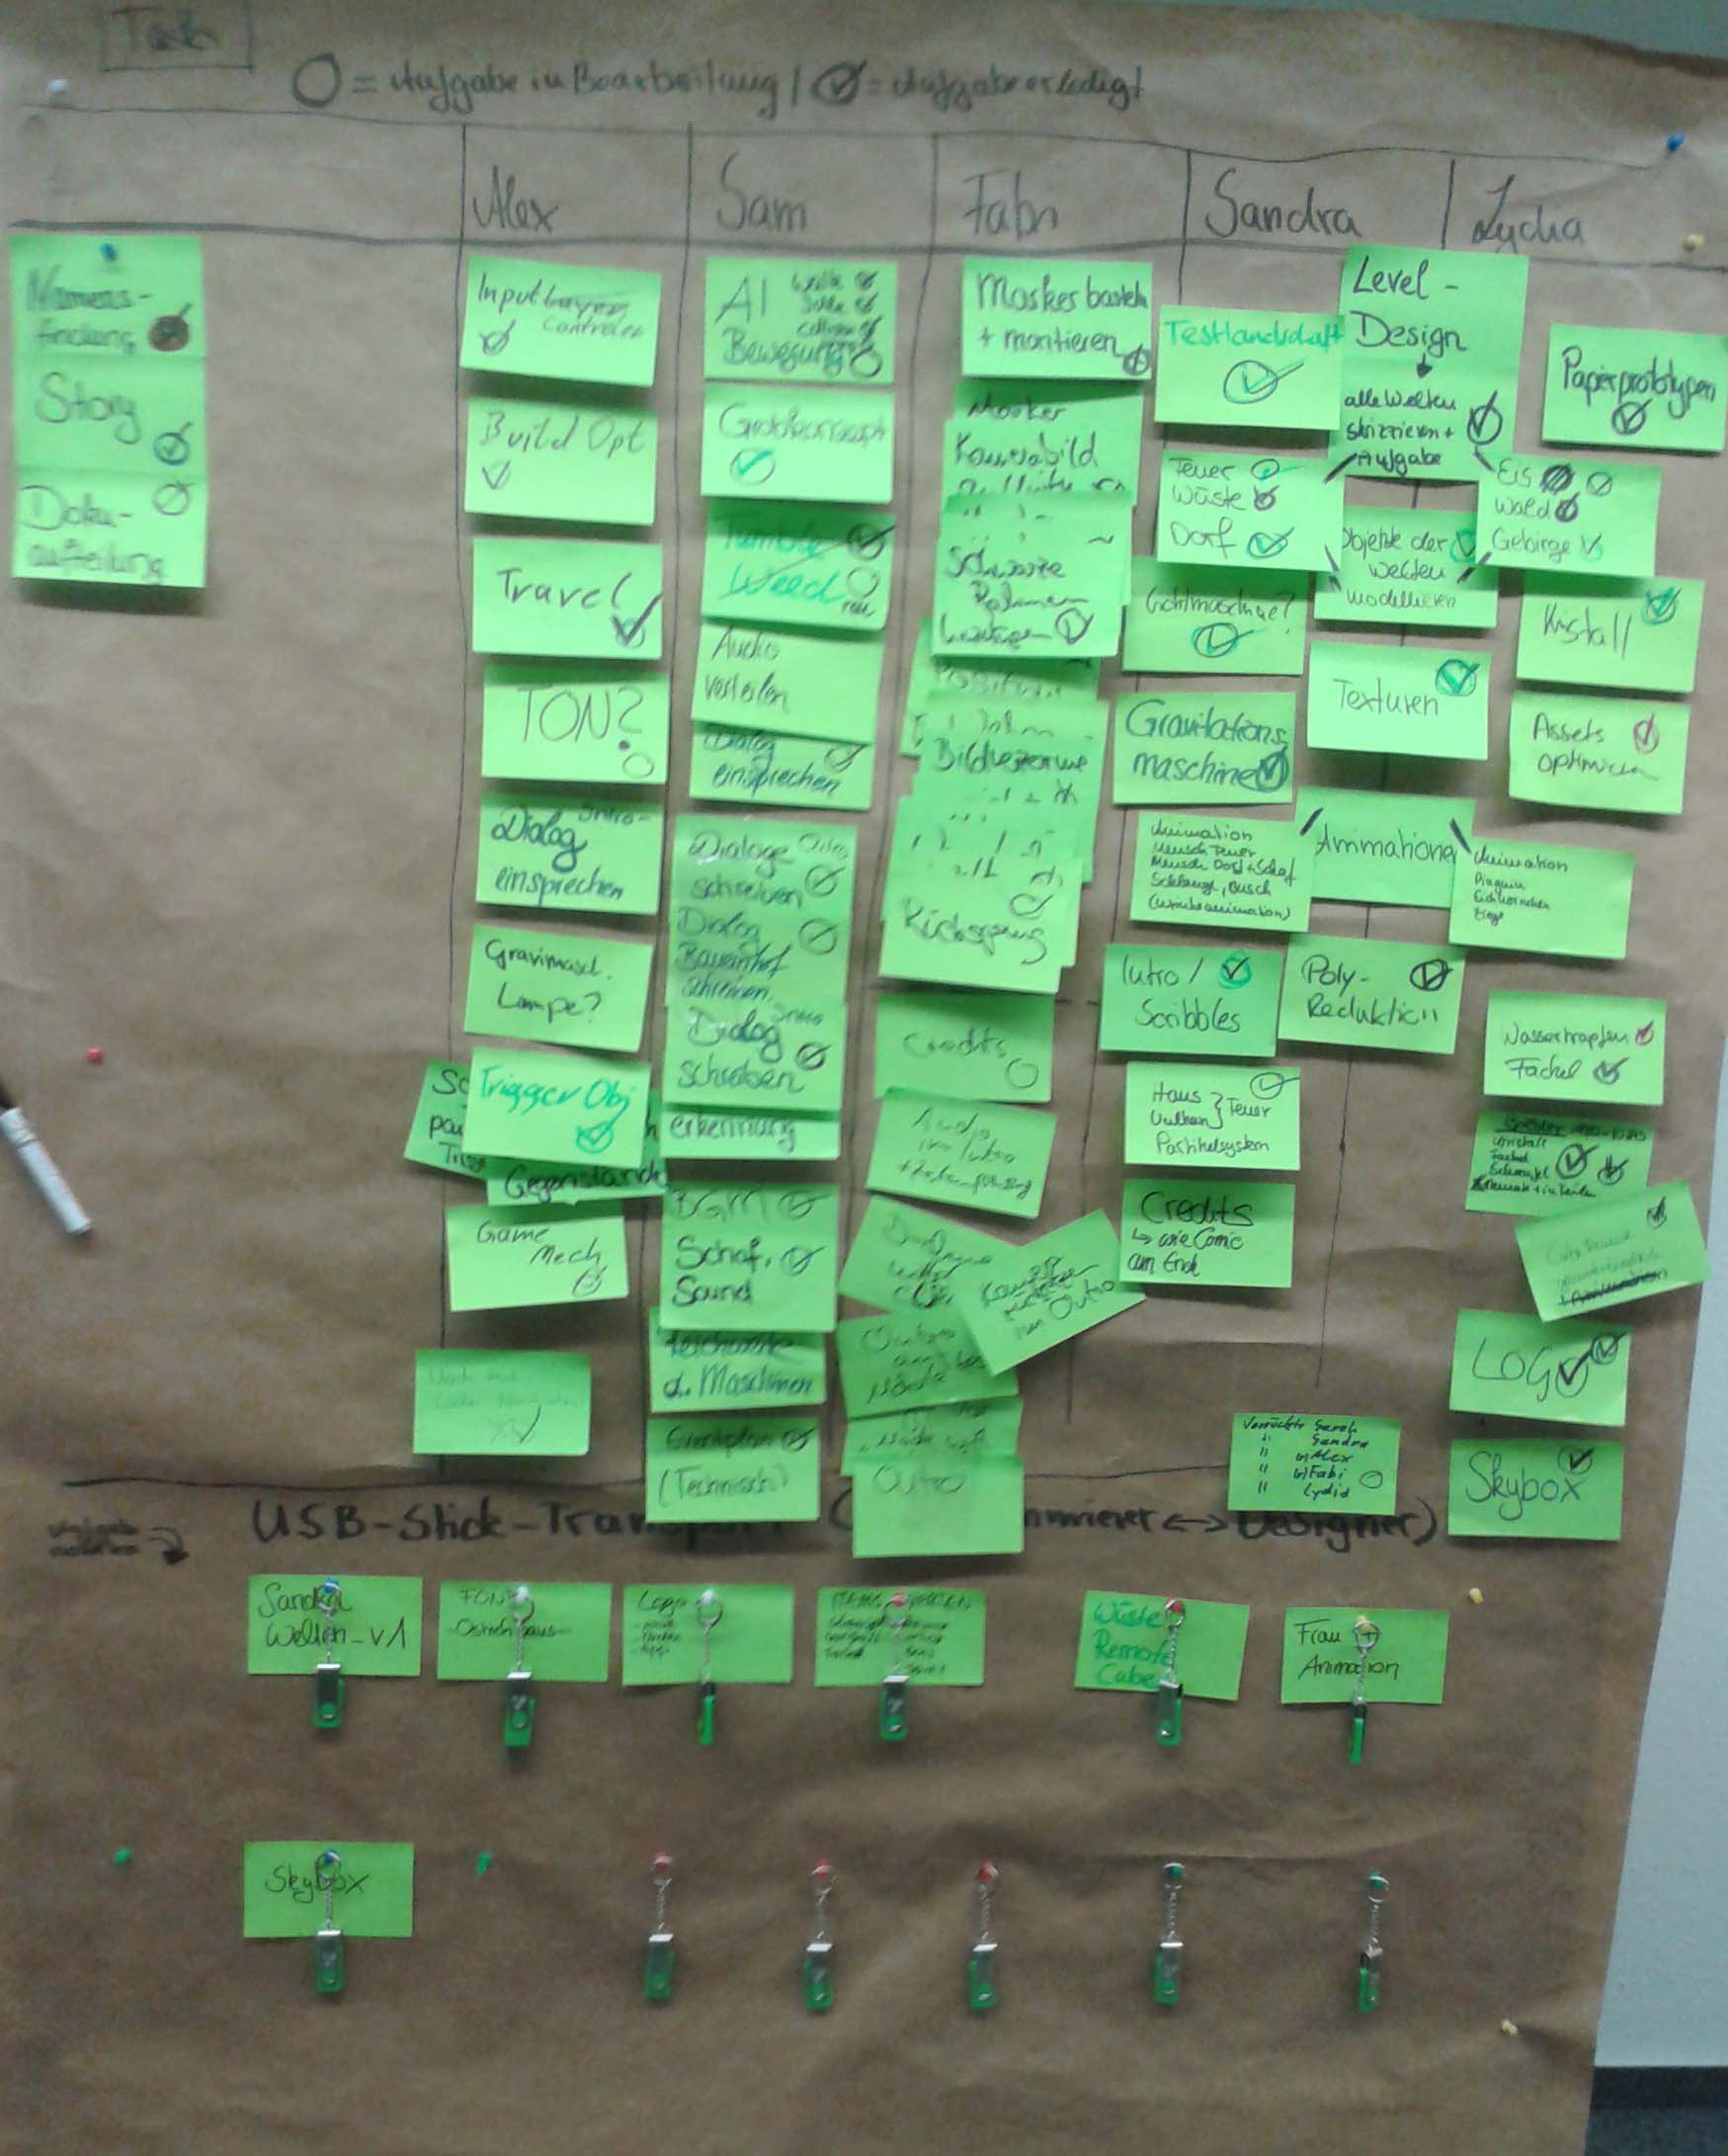
\includegraphics[width=1.0\textwidth]{images/Tasks}
	\caption{Taskboard}
	\label{fig:Tasks}
\end{figure}

Allgemeine Spieldesign-Entscheidungen wurden auf Whiteboards und Stehwänden erörtert und festgehalten. Daraus wurden Tasks gebildet, die auf einem Taskboard (siehe Abbildung \ref{fig:Tasks}) den einzelnen Teammitgliedern zugeordnet wurden. Angefangene und fertige Tasks wurden speziell markiert.

In tägliche kurzen Besprechungen am Morgen wurde festgelegt, welche Tasks bis zum Ende des Tages zu erfüllen sind (siehe Tabelle \ref{tab:Vorgehensweise}).

Einzelne Tasks wurden in Prototypen festgehalten und in eigenen Unity Szenen getestet. Das Projekt wurde durch Github versioniert. Notizen und das Designdokument wurden auf Google Drive geschrieben und in Latex zusammengefügt.

\begin{table}[!htbp]
\begin{center}
\begin{tabular}[hc]{l|l}
\hline
Mo & fertiges, grobes Konzept\\
& Welten und Aufgaben festlegen\\
& Markerprogrammierung\\
\hline
Di & Prototyp Papier\\
& Modellieren, Welten bauen\\
& Dialoge schreiben\\
& Grobkonzept\\
& 3D Tests der Welt\\
& Gamestates\\
\hline
Mi & Animationen\\
& Intro/Outro\\
& Gamestates und Trigger\\
& Dialoge einsprechen\\
& Sound\\
\hline
Do & Events finalisieren\\
& Outro mit Credits\\
& Doku beenden\\
\hline
Fr & Präsentation\\
\end{tabular}
\caption{Vorgehensweise}
\label{tab:Vorgehensweise}
\end{center}
\end{table}